\documentclass[12pt,a4paper]{report}
\usepackage[utf8]{inputenc}
\usepackage[spanish]{babel}
\usepackage{amsmath, amssymb}
\usepackage{graphicx}
\usepackage{geometry}
\usepackage{hyperref}
% Hipervínculos como texto coloreado (sin recuadros) usando el color institucional
\hypersetup{
    colorlinks=true,
    linkcolor=uoh,
    urlcolor=uoh,
    citecolor=uoh,
    filecolor=uoh
}
% URLs con el mismo estilo tipográfico que el texto
\urlstyle{same}
\usepackage{setspace}
\usepackage{xcolor}
\definecolor{uoh}{RGB}{79,131,198}


\geometry{left=3cm,right=2.5cm,top=2cm,bottom=2.5cm}
\setstretch{1.5}

\begin{document}

\begin{titlepage}
    \centering
    {
\includegraphics[width=0.3\textwidth]{data/logo.png}\par}
    {\normalsize\sffamily\textcolor{uoh}{Facultad de Ingeniería Civil en Computación}\par}
    \vspace{3cm}
    {\large\bfseries Desarrollo e implementación de una Plataforma Web Progresiva con Sincronización P2P para la Digitalización y Trazabilidad de Órdenes de Mantenimiento Industrial \par}
    \vspace{5cm}

    {\normalsize Autor: Yerko Ignacio Sepúlveda Rojas \par}
    {\normalsize Profesor Guía: Felipe Nicolas Gomez Molina \par}
    \vspace{4cm}
    {\normalsize Memoria para optar al título de Ingeniería Civil en Computación \par}
    \vfill
    {\normalsize Rancagua, Chile \par}
    {\normalsize Octubre, 2025 \par}
\end{titlepage}
\pagenumbering{roman} 
\tableofcontents
\listoffigures
\listoftables

\clearpage
\pagenumbering{arabic} % Números arábigos desde aquí

\chapter*{Introducción}
\addcontentsline{toc}{chapter}{Introducción}
\setcounter{page}{1}   % Empieza desde la página 1

En el entorno industrial actual, el mantenimiento preventivo y correctivo representa un factor crítico para garantizar la continuidad operacional y la optimización de recursos. Las empresas manufactureras enfrentan desafíos constantes relacionados con la planificación, ejecución y seguimiento de tareas de mantenimiento, especialmente cuando se trata de coordinar múltiple personal y gestiónar extensos procedimientos operativos.
El presente proyecto surge de la necesidad identificada en CARTOCOR, una empresa del sector industrial dedicada a la manufactura de cartón, donde se evidencia la ausencia de un sistema digitalizado para la gestión y seguimiento de ordenes de mantenimiento. La organización mantiene sus procedimientos operativos en formatos tradicionales (papel) con el apoyo de un servicio que no les da las herramientas requeridas (JD Edwards), lo que genera ineficiencia en la asignación de tareas, debido a que, la distribución manual de pautas de mantenimiento entre el personal resulta en tiempos muertos, mala gestión de cargas de trabajo y falta de visibilidad sobre el estado de las tareas. Tambien dificultad en el seguimiento en tiempo real sobre el estado de las tareas asignadas lo cual compromete la planificación operativa, los resultados de mantenimiento y la capacidad de respuesta ante imprevistos. Finalmente la inexistencia de trazabilidad en el tiempo impide hacer seguimiento a las órdenes de mantenimiento lo cual dificulta la identificación de patrones de fallas, el problema no siempre es de la máquina; también puede ser humano. Además la trazabilidad puede permitir identificar si los tiempos estimados se cumplen o no, y si es necesario ajustar los tiempos de las tareas de mantenimiento para ser mas realistas.

Debido a esto, la empresa requiere una plataforma que se adapte a sus necesidades operativas, que permita la digitalización de sus procedimientos de mantenimiento, la asignación eficiente de tareas, el seguimiento en tiempo real y la trazabilidad de las órdenes de mantenimiento, con ello buscar modernizar sus procesos y mejorar la planificación operativa.


\chapter*{Objetivos}
\addcontentsline{toc}{chapter}{Objetivos}

\section*{Objetivo General}
\addcontentsline{toc}{section}{Objetivos General}
Se busca como principal objetivo el desarrollar e implementar una Plataforma Web Progresiva (PWA) integrada con las plataformas existentes de CARTOCOR que digitalice los procedimientos de mantenimiento y optimice la planificación, asignación, ejecución, seguimiento y trazabilidad en tiempo real de órdenes y tareas, proporcionando soporte offline, colaboración entre supervisores y mantenedores, analítica histórica y capacidad de operación resiliente.
La aplicación utilizará una arquitectura modular compuesta por: frontend React, IndexedDB (Dexie) para persistencia local y operación offline, sincronización P2P con WebRTC y señalización vía Firebase Realtime Database, service worker para cacheo inteligente y actualización progresiva, generación y parsing de pautas en PDF (pdfjs-dist), y un esquema de versiones distribuido que garantice integridad y consistencia eventual en entornos con conectividad intermitente.

 
\newpage
\section*{Objetivo Específico}
\addcontentsline{toc}{section}{Objetivos Específico}

\begin{enumerate}
    \item Adaptar y digitalizar los procedimientos operativos de mantenimiento existentes en CARTOCOR, transformando los formatos tradicionales en un sistema digitalizado que permita una gestión más eficiente, segura y trazable.
    \item Implementar una red P2P utilizando WebRTC para la sincronización de datos entre dispositivos, permitiendo la colaboración en tiempo real entre supervisores y mantenedores, incluso en entornos con conectividad limitada.
    \item Desarrollar un modulo que procese las pautas existentes en formato PDF, extrayendo la información relevante para su almacenamiento y gestión dentro del sistema.
    \item Crear una interfaz web responsive utilizando tecnologías modernas que se adapte a múltiples dispositivos y proporcione una experiencia de usuario optimizada para entornos industriales.
    \item Desarrollar un módulo de gestión de pautas que permita la visualización, asignación, seguimiento y realizacion de procedimientos de mantenimiento.
    \item Establecer una arquitectura escalable que facilite futuras expansiones del sistema y la integración con otros sistemas empresariales.
\end{enumerate}

\chapter*{Hipótesis de Trabajo}
\addcontentsline{toc}{chapter}{Hipótesis de Trabajo}
La implementación de una solución tecnológica que se integre y adapte a las plataformas existentes dentro de la empresa en el area de mantenimiento de CARTOCOR permitirá mejorar significativamente la eficiencia operativa, la trazabilidad de las tareas y la planificación de mantenimiento, al proporcionar un sistema que optimiza la asignación de tareas, permitiendo el seguimiento en tiempo real y garantizando la seguridad de la información a través de una aplicacion web progresiva (PWA) con capacidades offline y colaboración en tiempo real.


\chapter*{Alcance}
\addcontentsline{toc}{chapter}{Alcance}
El sistema a desarrollar abarca la gestión completa del ciclo de vida de las órdenes de mantenimiento, desde su creación y asignación hasta su ejecución y trazabilidad en el tiempo. Se incluye la implementación de una red P2P desentralizada con almacenamiento redundante y jerarquico en los dispositivos de la red, flujo de datos entre los peers y generacion de informes respectivo a los datos. La aplicación será accesible desde dispositivos móviles y de escritorio, adaptándose a las necesidades operativas de los usuarios en el entorno industrial. Se implementará un sistema de autenticación y autorización para garantizar la seguridad y privacidad de los datos, así como mecanismos de respaldo y recuperación ante fallos.  La aplicación estará diseñada para operar en entornos con conectividad intermitente, utilizando almacenamiento local y sincronización P2P para asegurar la continuidad operativa. Se desarrollará una interfaz de usuario intuitiva y fácil de usar, con funcionalidades específicas para supervisores y mantenedores. Se proporcionará soporte para la generación y visualización de informes históricos y analíticos sobre las órdenes de mantenimiento.
\newline
El proyecto no incluye la integración directa con sistemas ERP existentes, aunque la arquitectura estara diseñada para un facil acoplamiente con las plataformas existentes en Cartocor, de esta manera poder ser utilizada como complemento.

\chapter*{Marco Teórico}
\addcontentsline{toc}{chapter}{Marco Teórico}

\section*{Gestión del mantenimiento industrial}
La gestión del mantenimiento se enmarca dentro de la disciplina de la ingeniería de confiabilidad, la cual busca maximizar la disponibilidad de los activos productivos optimizando recursos humanos y materiales. Conceptos como Mantenimiento Centrado en Confiabilidad (RCM), Total Productive Maintenance (TPM) y mantenimiento predictivo orientan la identificación de criticidades, la priorización de intervenciones y la medición de indicadores clave (MTBF, MTTR, OEE). Estos enfoques constituyen la base operativa sobre la que se articula la digitalización propuesta.

\subsection*{Digitalización de procesos de mantenimiento}
La migración desde flujos manuales hacia sistemas digitales implica modelar procedimientos, trazabilidad documental y gobernanza de datos. Las arquitecturas empresariales contemporáneas incorporan capas de integración con sistemas ERP y plataformas de analítica, donde la interoperabilidad y el cumplimiento normativo (ISO 55000, ISO 14224)\cite{iso55000:2014,iso14224:2016} resultan determinantes para consolidar repositorios de conocimiento y reducir el riesgo operativo.

\section*{Transformación digital e Industria 4.0}
El paradigma de Industria 4.0 habilita fábricas conectadas capaces de intercambiar información en tiempo real. Tecnologías como Internet of Things (IoT), ciberfísicos y analítica avanzada permiten visualizar estados operacionales y anticipar fallas. La propuesta se alinea con estos principios al introducir una plataforma colaborativa, resiliente y móvil que soporta sincronización distribuida y operación offline para entornos con conectividad intermitente.

\section*{Aplicaciones web progresivas (PWA)}
Las PWA combinan capacidades de aplicaciones nativas con la ubicuidad de la web mediante el uso de Service Workers, Application Shell Architecture y Web App Manifests. Estos componentes permiten cacheo inteligente, notificaciones push y actualizaciones progresivas, garantizando continuidad de servicio y experiencia de usuario consistente. En contextos industriales, las PWA facilitan despliegues controlados, disminuyen costos de mantenimiento y aseguran compatibilidad con diferentes dispositivos.

\subsection*{Persistencia local y operación offline}
IndexedDB constituye el estándar para almacenamiento estructurado en navegadores, soportando transacciones y consultas asincrónicas. Bibliotecas como Dexie abstraen la complejidad de la API nativa y proveen mecanismos de versionado, migraciones y notificaciones de cambio. Estas capacidades son esenciales para registrar órdenes de trabajo, controles de checklist y evidencias fotográficas cuando la red es inestable.

\section*{Sincronización distribuida y colaboración en tiempo real}
La sincronización P2P basada en WebRTC posibilita el intercambio directo de datos entre clientes sin pasar por servidores intermedios, reduciendo latencias y habilitando tolerancia a fallos. La señalización mediada por servicios como Firebase Realtime Database establece los canales de comunicación, mientras que patrones de replicación eventual y estructuras de datos convergentes (CRDT) aseguran consistencia pese a desconexiones temporales. El diseño requiere políticas de versionado, reconciliación de conflictos y registros de auditoría.

\section*{WebRTC y Redes P2P para Sincronización de Datos}
Web Real-Time Communication (WebRTC) es un conjunto de especificaciones y APIs que habilita comunicaciones de baja latencia (audio, video y datos arbitrarios) directamente entre navegadores y otras aplicaciones compatibles. Su adopción en aplicaciones de mantenimiento industrial se justifica por: (i) reducción de dependencia en servidores centrales, (ii) resiliencia ante fallos de conectividad parcial, (iii) menor latencia en la propagación de cambios operativos y (iv) escalabilidad horizontal basada en los propios dispositivos de la planta.

\subsection*{Arquitectura lógica de WebRTC}
Un canal WebRTC se establece en tres fases: negociación de sesión (oferta/respuesta SDP), descubrimiento de rutas (recolección e intercambio de candidatos ICE) y establecimiento seguro de canales (DTLS-SRTP para medios y DTLS sobre SCTP para datos). La plataforma se apoya en un servicio de señalización externo (Firebase Realtime Database) exclusivamente para intercambiar metadatos de sesión, evitando transportar la carga útil por la infraestructura central.

\subsection*{Mecanismo ICE y candidatos de conectividad}
Interactive Connectivity Establishment (ICE) coordina la comprobación de pares potenciales de transporte combinando direcciones locales (host), reflejadas (STUN) y de retransmisión (TURN). En entornos corporativos con NAT simétricos o firewalls restrictivos, la disponibilidad de un servidor TURN es determinante para garantizar conectividad. La priorización dinámica de candidatos optimiza latencia y estabilidad de la sesión.

\subsection*{Rol de STUN y TURN}
Los servidores STUN proporcionan la dirección pública del cliente para facilitar la conectividad directa, mientras que TURN retransmite el tráfico cuando la conexión peer-to-peer directo resulta inviable. El diseño balancea costo y disponibilidad limitando el uso de TURN a escenarios de bloqueo estricto, preservando así eficiencia de ancho de banda.

\subsection*{Data Channels y SCTP}
Los DataChannels de WebRTC utilizan SCTP encapsulado sobre DTLS, ofreciendo modos confiables y no confiables, ordenados o desordenados. Esta flexibilidad permite adaptar la entrega de mensajes: para metadatos críticos (versiones, confirmaciones) se usa un canal confiable y ordenado; para actualizaciones incrementales o notificaciones no críticas se puede optar por canales no confiables que reducen latencia al evitar retransmisiones excesivas.

\subsection*{Modelos de consistencia y resolución de conflictos}
La naturaleza distribuida de la red exige estrategias de consistencia eventual. Se emplean números de versión monótonos y marcas temporales lógicas para ordenar operaciones. Para colecciones estructuradas se considerarían CRDTs (por ejemplo, mapas de última escritura ganadora - LWW) si la complejidad de conflictos creciera. La política local actual prioriza: (1) versión mayor, (2) igualdad de versión: última marca temporal, (3) igualdad completa: descartar duplicado.

\subsection*{Topologías y escalabilidad}
Aunque WebRTC facilita mallas completas (full-mesh), el crecimiento cuadrático de conexiones (complejidad $O(n^2)$) limita su escalabilidad. Para el caso de uso (número moderado de supervisores y mantenedores) una malla controlada es suficiente. Futuras extensiones podrían incorporar \textit{super-peers} (nodos con mayores capacidades) para agregación de snapshots o un enfoque jerárquico/árbol parcial que reduzca la sobrecarga a aproximaciones más cercanas a $O(n)$ en la distribución de estados agregados.

\subsection*{Seguridad y cifrado de extremo a extremo}
WebRTC cifra todos los canales utilizando DTLS, proporcionando confidencialidad e integridad. Se añaden controles de acceso a nivel de señalización (tokens y roles) que inhiben intentos de unión no autorizados. Las políticas de rotación de sesión y invalidación de credenciales reducen la ventana de explotación si se expone un identificador de sala o canal de señalización.

\subsection*{Limitaciones y mitigaciones}
Entre las limitaciones se encuentran: (i) variabilidad de ruteo bajo NAT que causa reconexiones, (ii) consumo incremental de CPU en mallas densas, (iii) complejidad de depuración en rutas TURN y (iv) ausencia de almacenamiento histórico centralizado inmediato. Se mitiga mediante: reconexión exponencial, compresión y batching de cambios, monitoreo de métricas de sesión y periodicidad de snapshots para persistencia redundante.

\subsection*{Justificación en el contexto de mantenimiento}
La elección de WebRTC reduce el riesgo de interrupción global al distribuir la responsabilidad de sincronización. Supervisores pueden continuar coordinando tareas y registrando evidencias aun cuando el enlace a Internet sea intermitente, propagando los cambios cuando se restablezcan rutas P2P o mediante reenvío diferido a través de pares disponibles.

\subsection*{Comparación con alternativas}
En contraste con enfoques centralizados (REST polling, WebSockets a un servidor único), WebRTC minimiza single points of failure y latencias inducidas por hubs. Frente a soluciones de replicación eventual basadas sólo en sincronización diferida (por ejemplo, colas offline + reenvío), la capa P2P ofrece visibilidad inmediata de estado operativo, mejorando la coordinación táctica en planta.

\subsection*{Jerarquías de acceso y control de roles}
Los modelos de control de acceso basado en roles (RBAC) permiten delimitar permisos para supervisores, mantenedores y administradores. La correcta implementación del RBAC garantiza segregación de funciones, soporte a flujos de aprobación y trazabilidad de cambios, requisitos críticos en plantas productivas sujetas a auditorías internas y externas.

\section*{Experiencia de usuario y ergonomía digital}
El diseño centrado en el usuario (UCD) y la ingeniería de usabilidad aseguran interfaces intuitivas, reducen tiempos de entrenamiento y disminuyen errores operativos.

\section*{Analítica y toma de decisiones basada en datos}
La integración de analítica descriptiva, diagnóstica y predictiva sobre los datos de mantenimiento habilita tableros de control, proyecciones de costo y evaluación de desempeño. Tecnologías de Business Intelligence y aprendizaje automático aportan modelos de pronóstico, detección de anomalías y recomendación de acciones correctivas, todo ello sustentado en la calidad y disponibilidad de la información capturada por la plataforma.

\section*{Regulaciones y estándares aplicables}
Los desarrollos tecnológicos en plantas industriales deben alinearse con marcos regulatorios de seguridad laboral, gestión de activos y protección de datos personales. Normativas como ISO 45001, ISO\/IEC 27001 y legislaciones de privacidad (por ejemplo, Ley 19.628 en Chile)\cite{iso45001:2018,iso27001:2022,ley19628} condicionan el diseño de controles técnicos y organizacionales, asegurando cumplimiento y confianza de las partes interesadas.


\chapter*{Metodología de Investigación y Desarrollo}
\addcontentsline{toc}{chapter}{Metodología de Investigación y Desarrollo}
\section*{Tipo y enfoque de la investigación} La investigación es de tipo aplicada y adopta un enfoque mixto: cualitativo en el levantamiento y análisis de procesos de mantenimiento existentes, y cuantitativo en la evaluación de métricas de desempeño (latencia de sincronización, disponibilidad offline, tiempo medio de registro de tareas y resolución de conflictos de datos).

\section*{Metodología general: Design Science Research} 
Se sigue el paradigma Design Science Research (DSR) \cite{hevner2004,peffers2007}, abordando seis pasos: (1) identificación del problema, (2) definición de objetivos de solución, (3) diseño del artefacto, (4) construcción, (5) evaluación iterativa y (6) comunicación de resultados. El artefacto central es una plataforma PWA con sincronización P2P que digitaliza y traza órdenes de mantenimiento.

\section*{Estrategia de desarrollo iterativo–incremental} El desarrollo se organiza en iteraciones cortas (2–3 semanas) aplicando principios ágiles: backlog evolutivo, priorización por valor de riesgo, prototipado temprano y refactorización continua. No se adopta un framework formal completo (Scrum) dado el carácter monousuario del equipo de desarrollo.

\section*{Fases del proceso} 
\begin{enumerate} 
    \item Relevamiento y análisis: entrevistas exploratorias, revisión de procedimientos actuales y mapeo de flujos manuales. 
    
    \item Definición de requerimientos: clasificación en funcionales (gestión de órdenes, sincronización P2P, operación offline) y no funcionales (disponibilidad, consistencia eventual, seguridad, usabilidad). 

    \item Diseño arquitectónico: selección tecnológica (React, IndexedDB via Dexie, WebRTC, Firebase RTDB para señalización, service workers). 

    \item Construcción incremental: implementación de módulos núcleo (auth local, almacenamiento, procesamiento del PDF, canal P2P, versionado). 

    \item Evaluación iterativa: pruebas funcionales, ensayos de desconexión/reconexión, medición de latencia y análisis de conflictos de datos. 

    \item Optimización y refactorización: mejoras en jerarquía de roles, batching de sincronización, ergonomía de UI. 

    \item Validación final: consolidación de métricas y contrastación con objetivos definidos. 
\end{enumerate}

\section*{Instrumentos y técnicas}

Observación de procesos de mantenimiento existentes.
Análisis documental (pautas en PDF).
Pruebas de caja negra y escenarios offline.
Mediciones de tiempo (latencia P2P, tiempo de carga inicial, tiempo de parse de PDF).
Registro de conflictos y resolución (log de versiones y reconciliaciones).

\section*{Criterios de evaluación} Se adoptan atributos de calidad inspirados en ISO/IEC 25010\cite{iso25010:2011}: funcionalidad, fiabilidad (consistencia eventual y manejo de desconexiones), eficiencia de desempeño (tiempo de sincronización), usabilidad (flujo de tareas), mantenibilidad (modularidad) y seguridad (aislamiento de roles, cifrado en tránsito).

\section*{Métricas clave} \begin{itemize} \item Latencia media de propagación de cambios P2P (ms). \item Tasa de éxito de operaciones offline (\% operaciones almacenadas y sincronizadas sin pérdida). \item Tasa de conflictos por 100 sincronizaciones. \item Tiempo medio de parse de una pauta PDF (s). \item Peso de assets iniciales (KB) y tiempo de carga en primer y segundo arranque (frío / caliente). \end{itemize}

\section*{Gestión de riesgos} Riesgos abordados: (i) conectividad intermitente (mitigado con almacenamiento local y reintentos exponenciales), (ii) conflicto de versiones (versionado monótono y reglas de resolución), (iii) saturación de malla P2P (limitación de peers simultáneos y potencial diseño jerárquico), (iv) inconsistencia en parse de PDFs (validaciones y logs de errores).

\section*{Consideraciones éticas y de seguridad} Protección de datos operativos mediante control de roles, minimización de superficie de ataque (no exponer endpoints innecesarios) y cifrado end-to-end de canales WebRTC.

\chapter*{Resultados}


\chapter*{Conclusiones}


\appendix
\chapter*{Apéndice}
\addcontentsline{toc}{chapter}{Apéndice}
\section*{Implementación de Plataforma}
\subsection*{Mantenedor}
\begin{figure}[h]
    \centering
    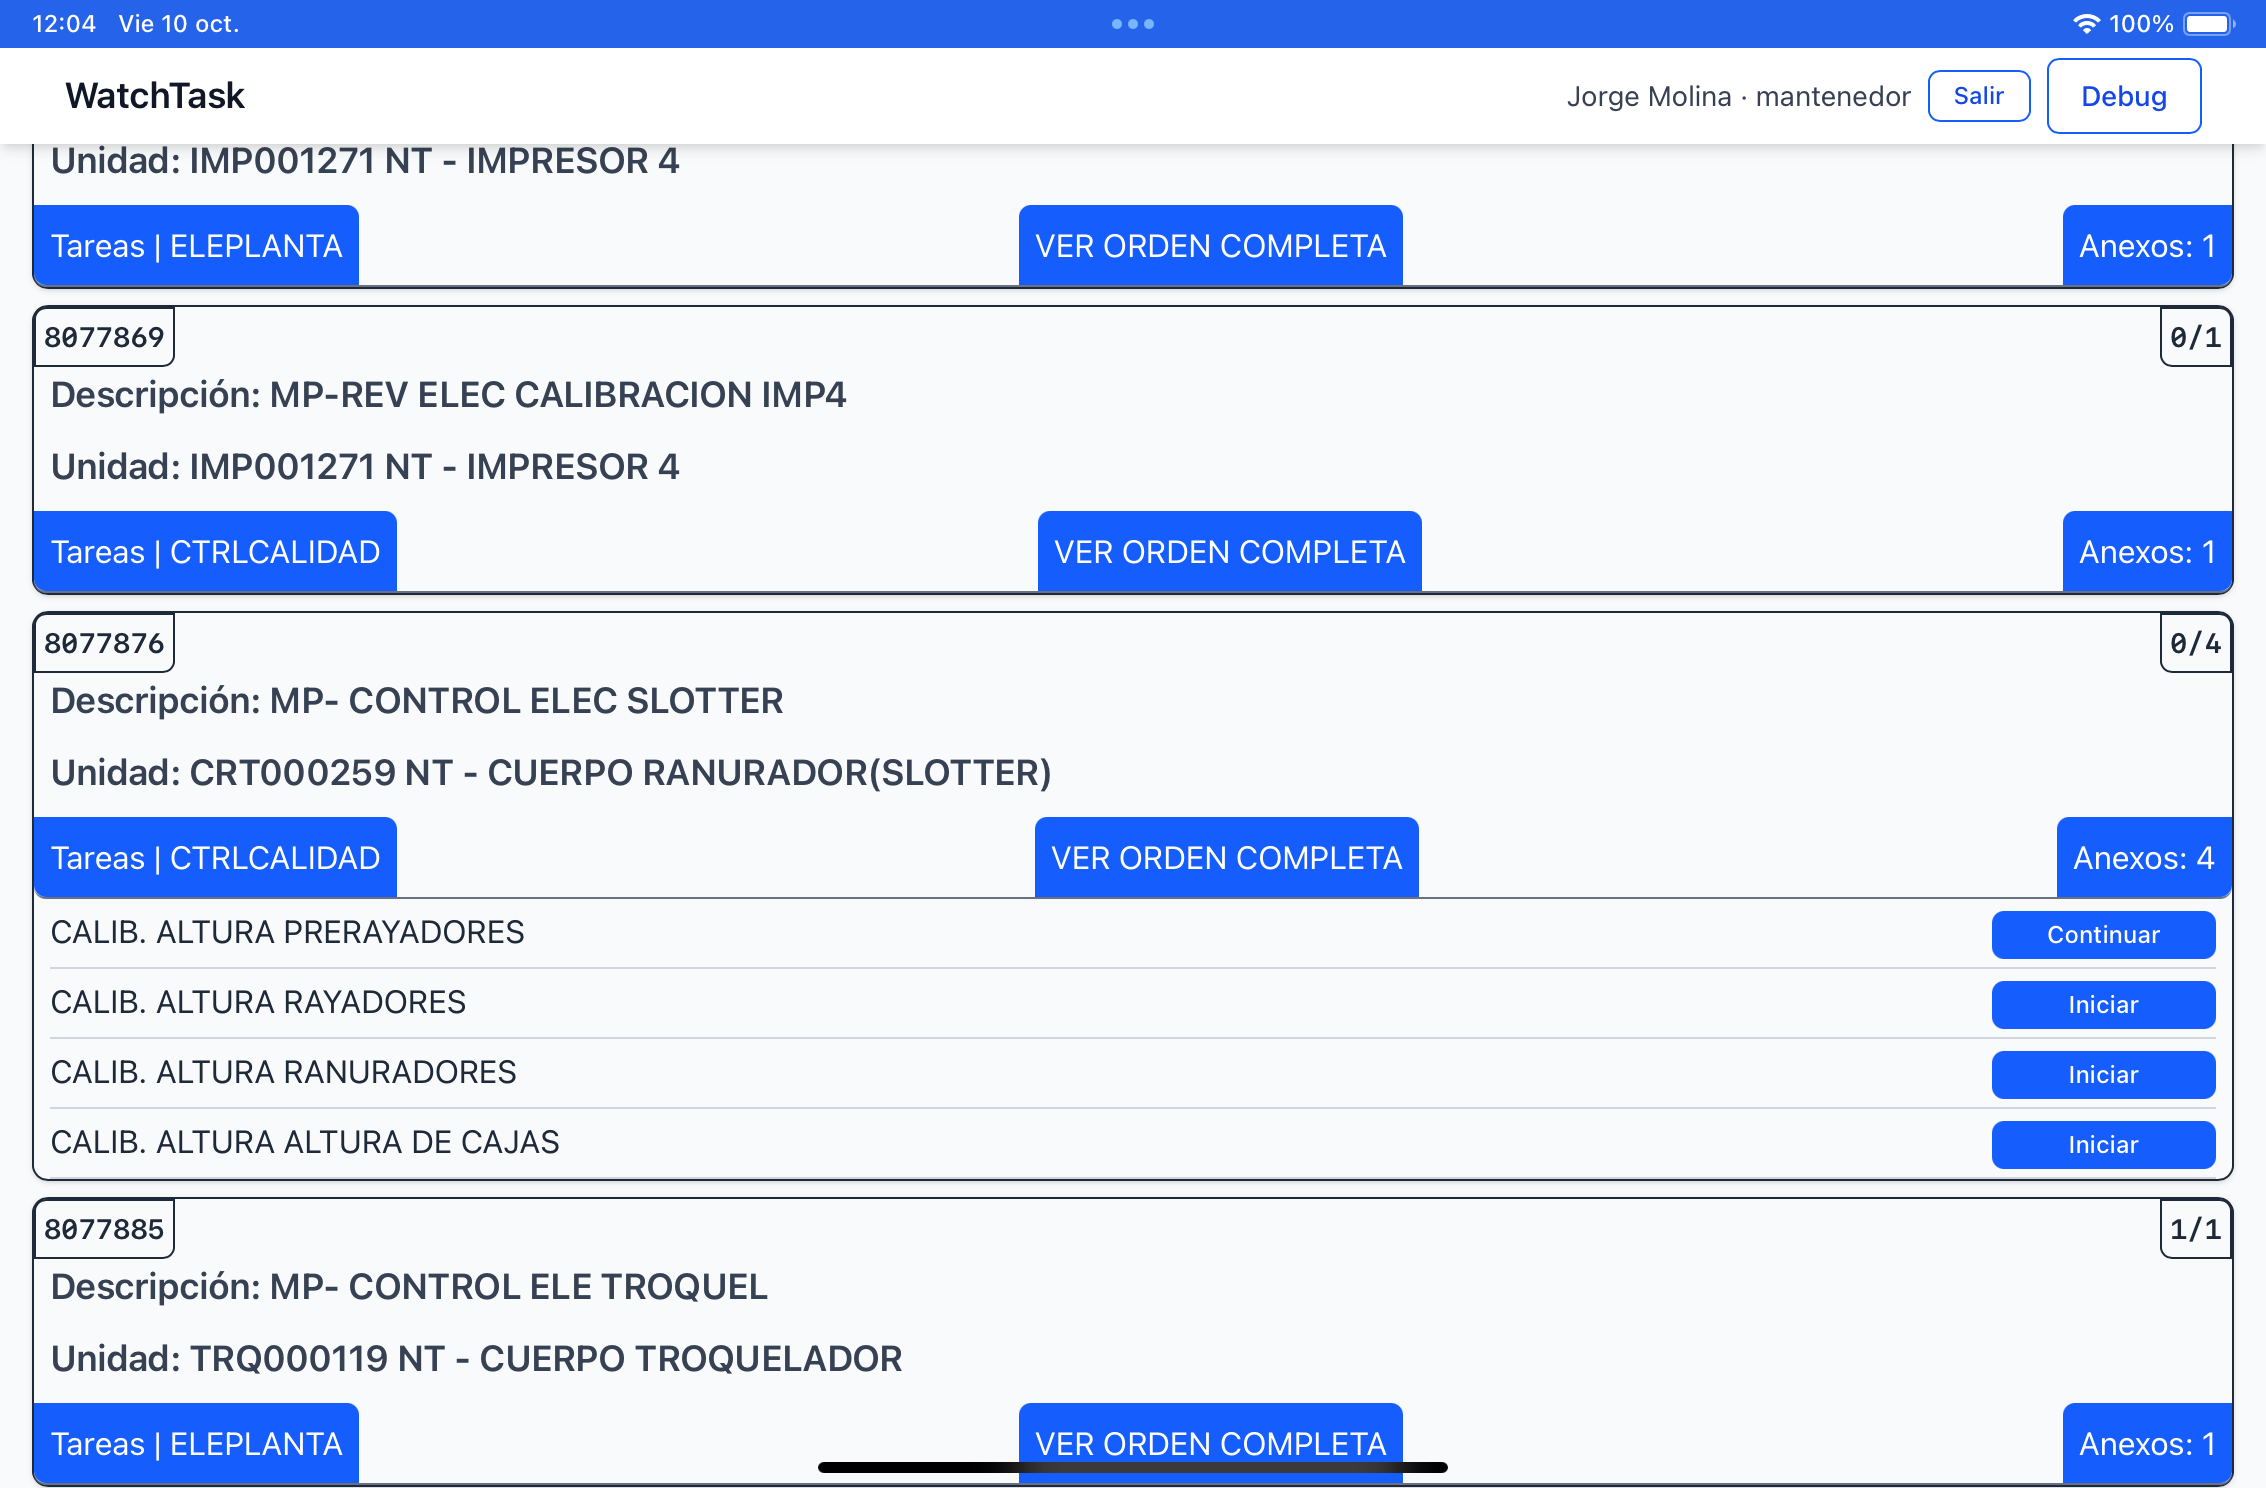
\includegraphics[width=1\textwidth]{data/Mantenedor_HOME_task.png}
    \caption[\,Mantenedor: Vista inicial (tareas)]{Interfaz de usuario con perfil Mantenedor, Vista Inicial, segmento de tareas expandido.}
    \label{fig:[Mantenedor_HOME_task]}
\end{figure}
\begin{figure}[h]
    \centering
    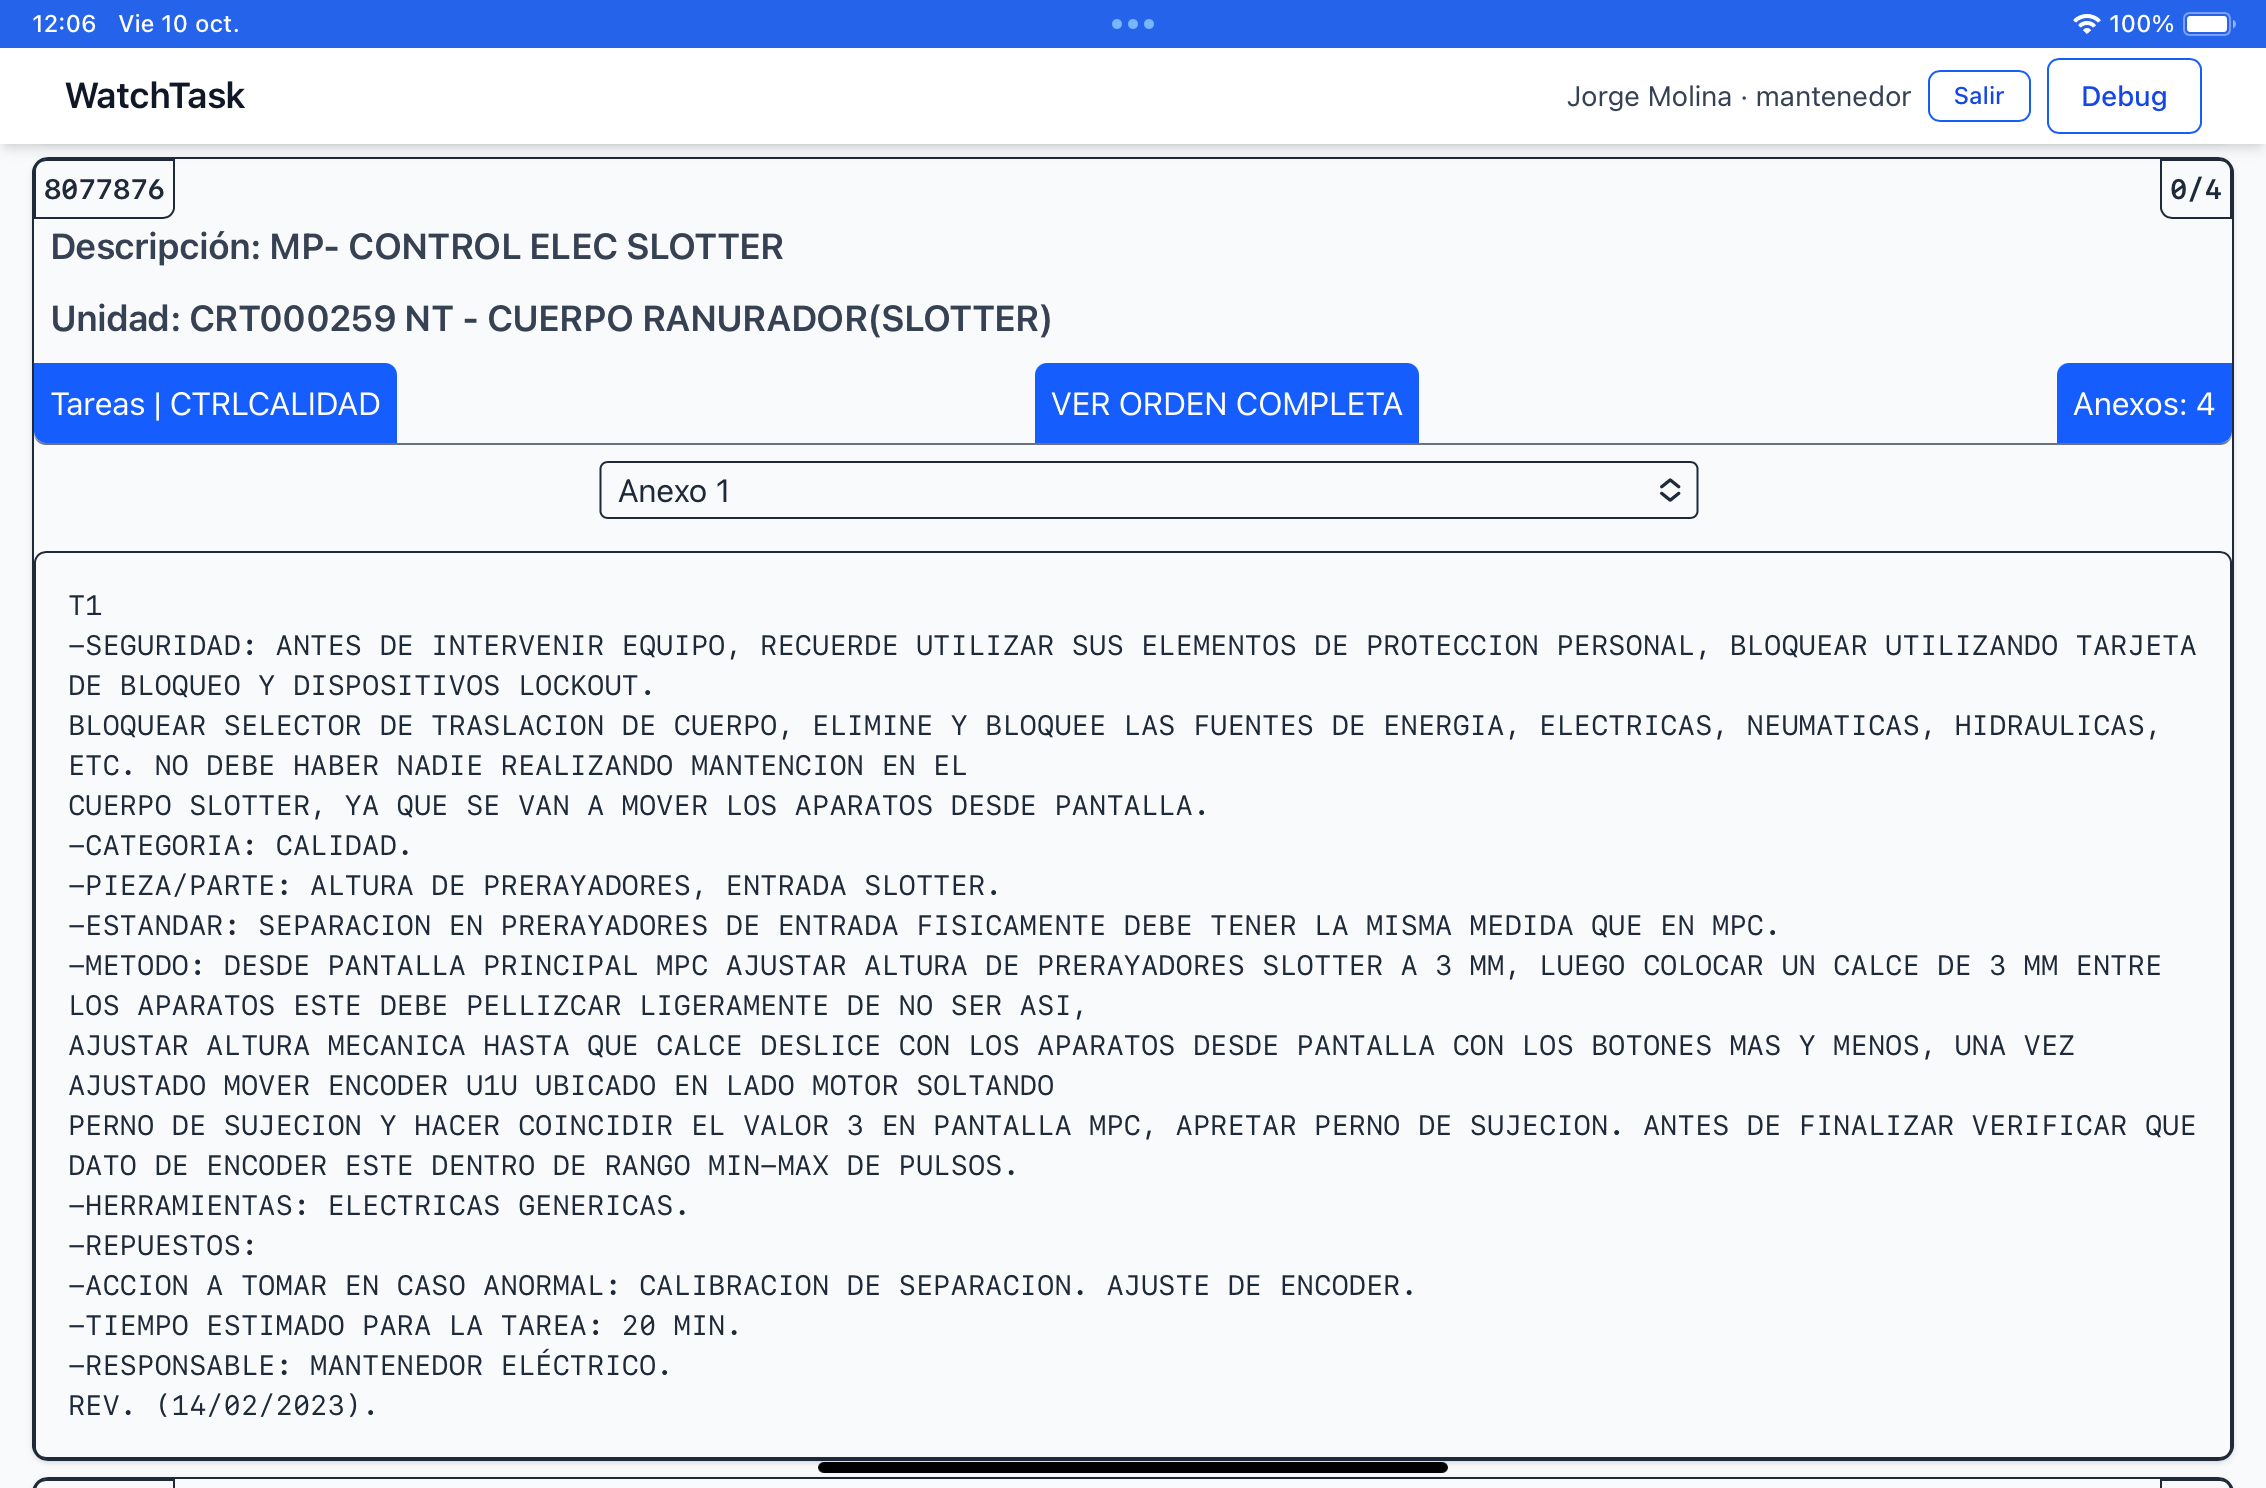
\includegraphics[width=1\textwidth]{data/Mantenedor_HOME_anexo.png}
    \caption[\,Mantenedor: Vista inicial (anexos)]{Interfaz de usuario con perfil Mantenedor, Vista Inicial, segmento de anexos expandido.}
    \label{fig:[Mantenedor_HOME_anexo]}
\end{figure}
\begin{figure}[h]
    \centering
    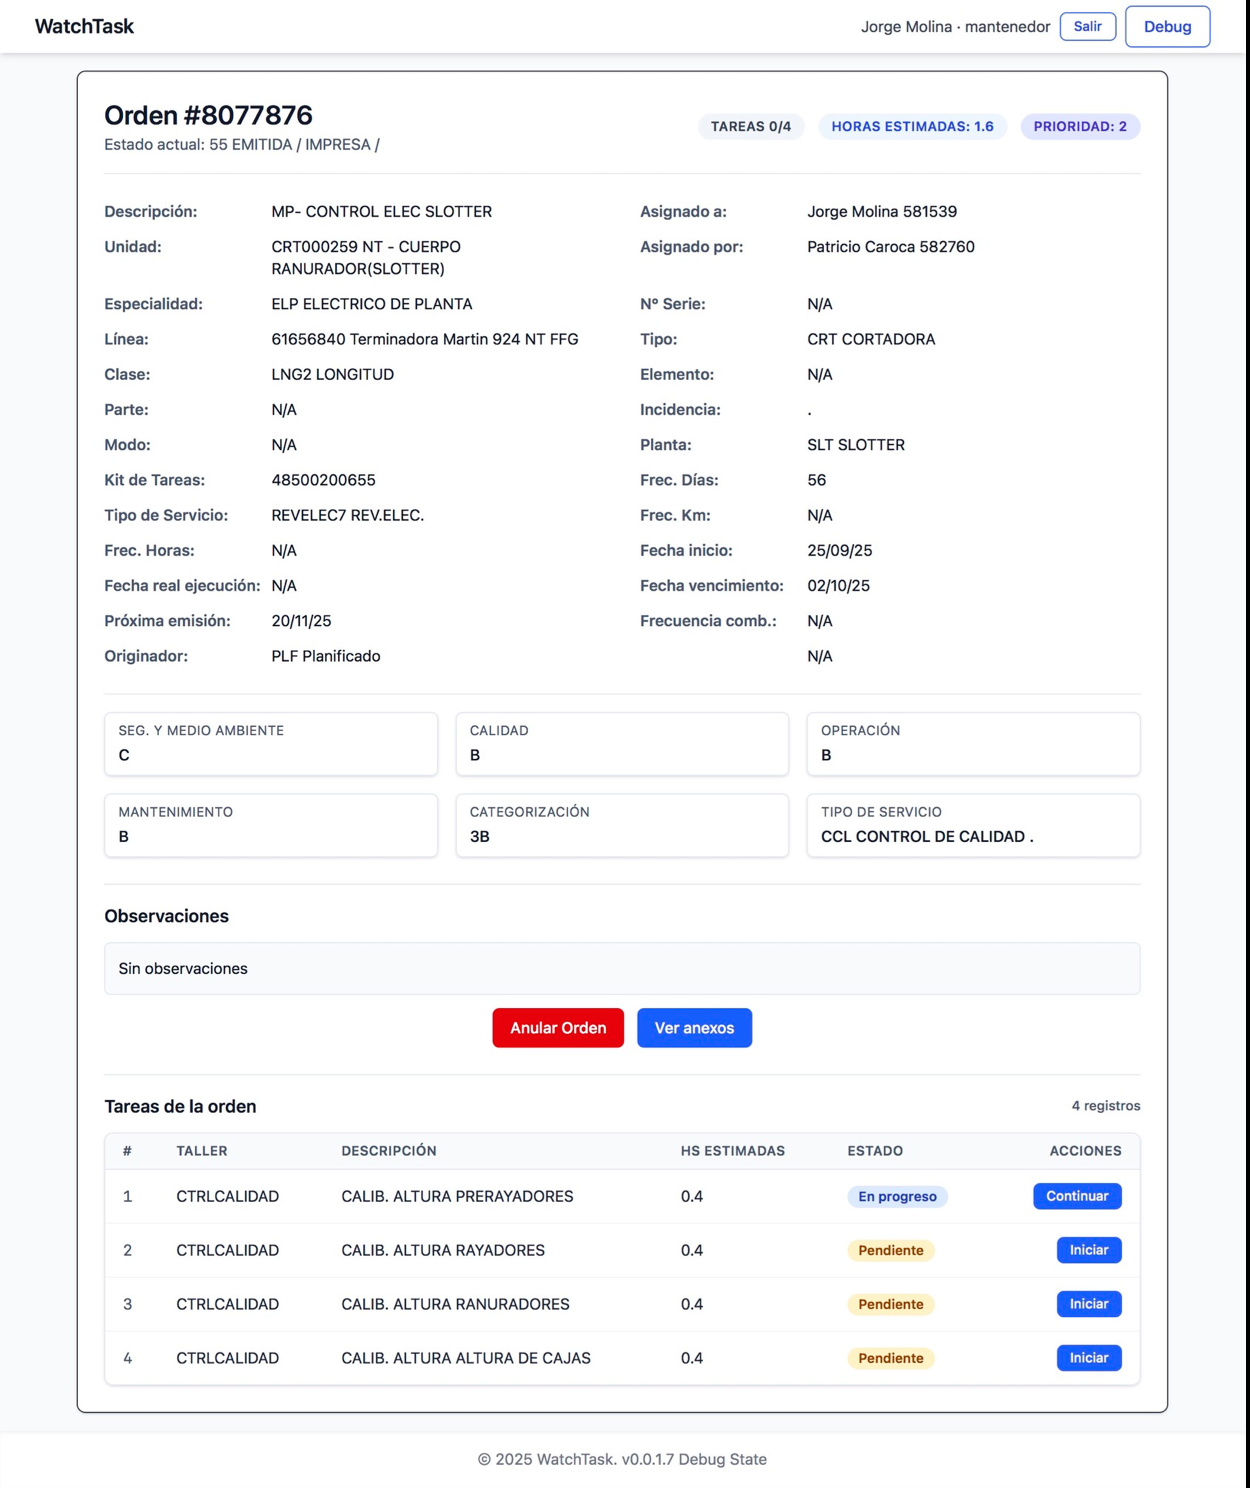
\includegraphics[width=1\textwidth]{data/Mantenedor_Orden.png}
    \caption[\,Mantenedor: Vista de Orden]{Interfaz de usuario con perfil Mantenedor, Vista de Orden de Mantenimiento.}
    \label{fig:[Mantenedor_Orden]}
\end{figure}
\begin{figure}[h]
    \centering
    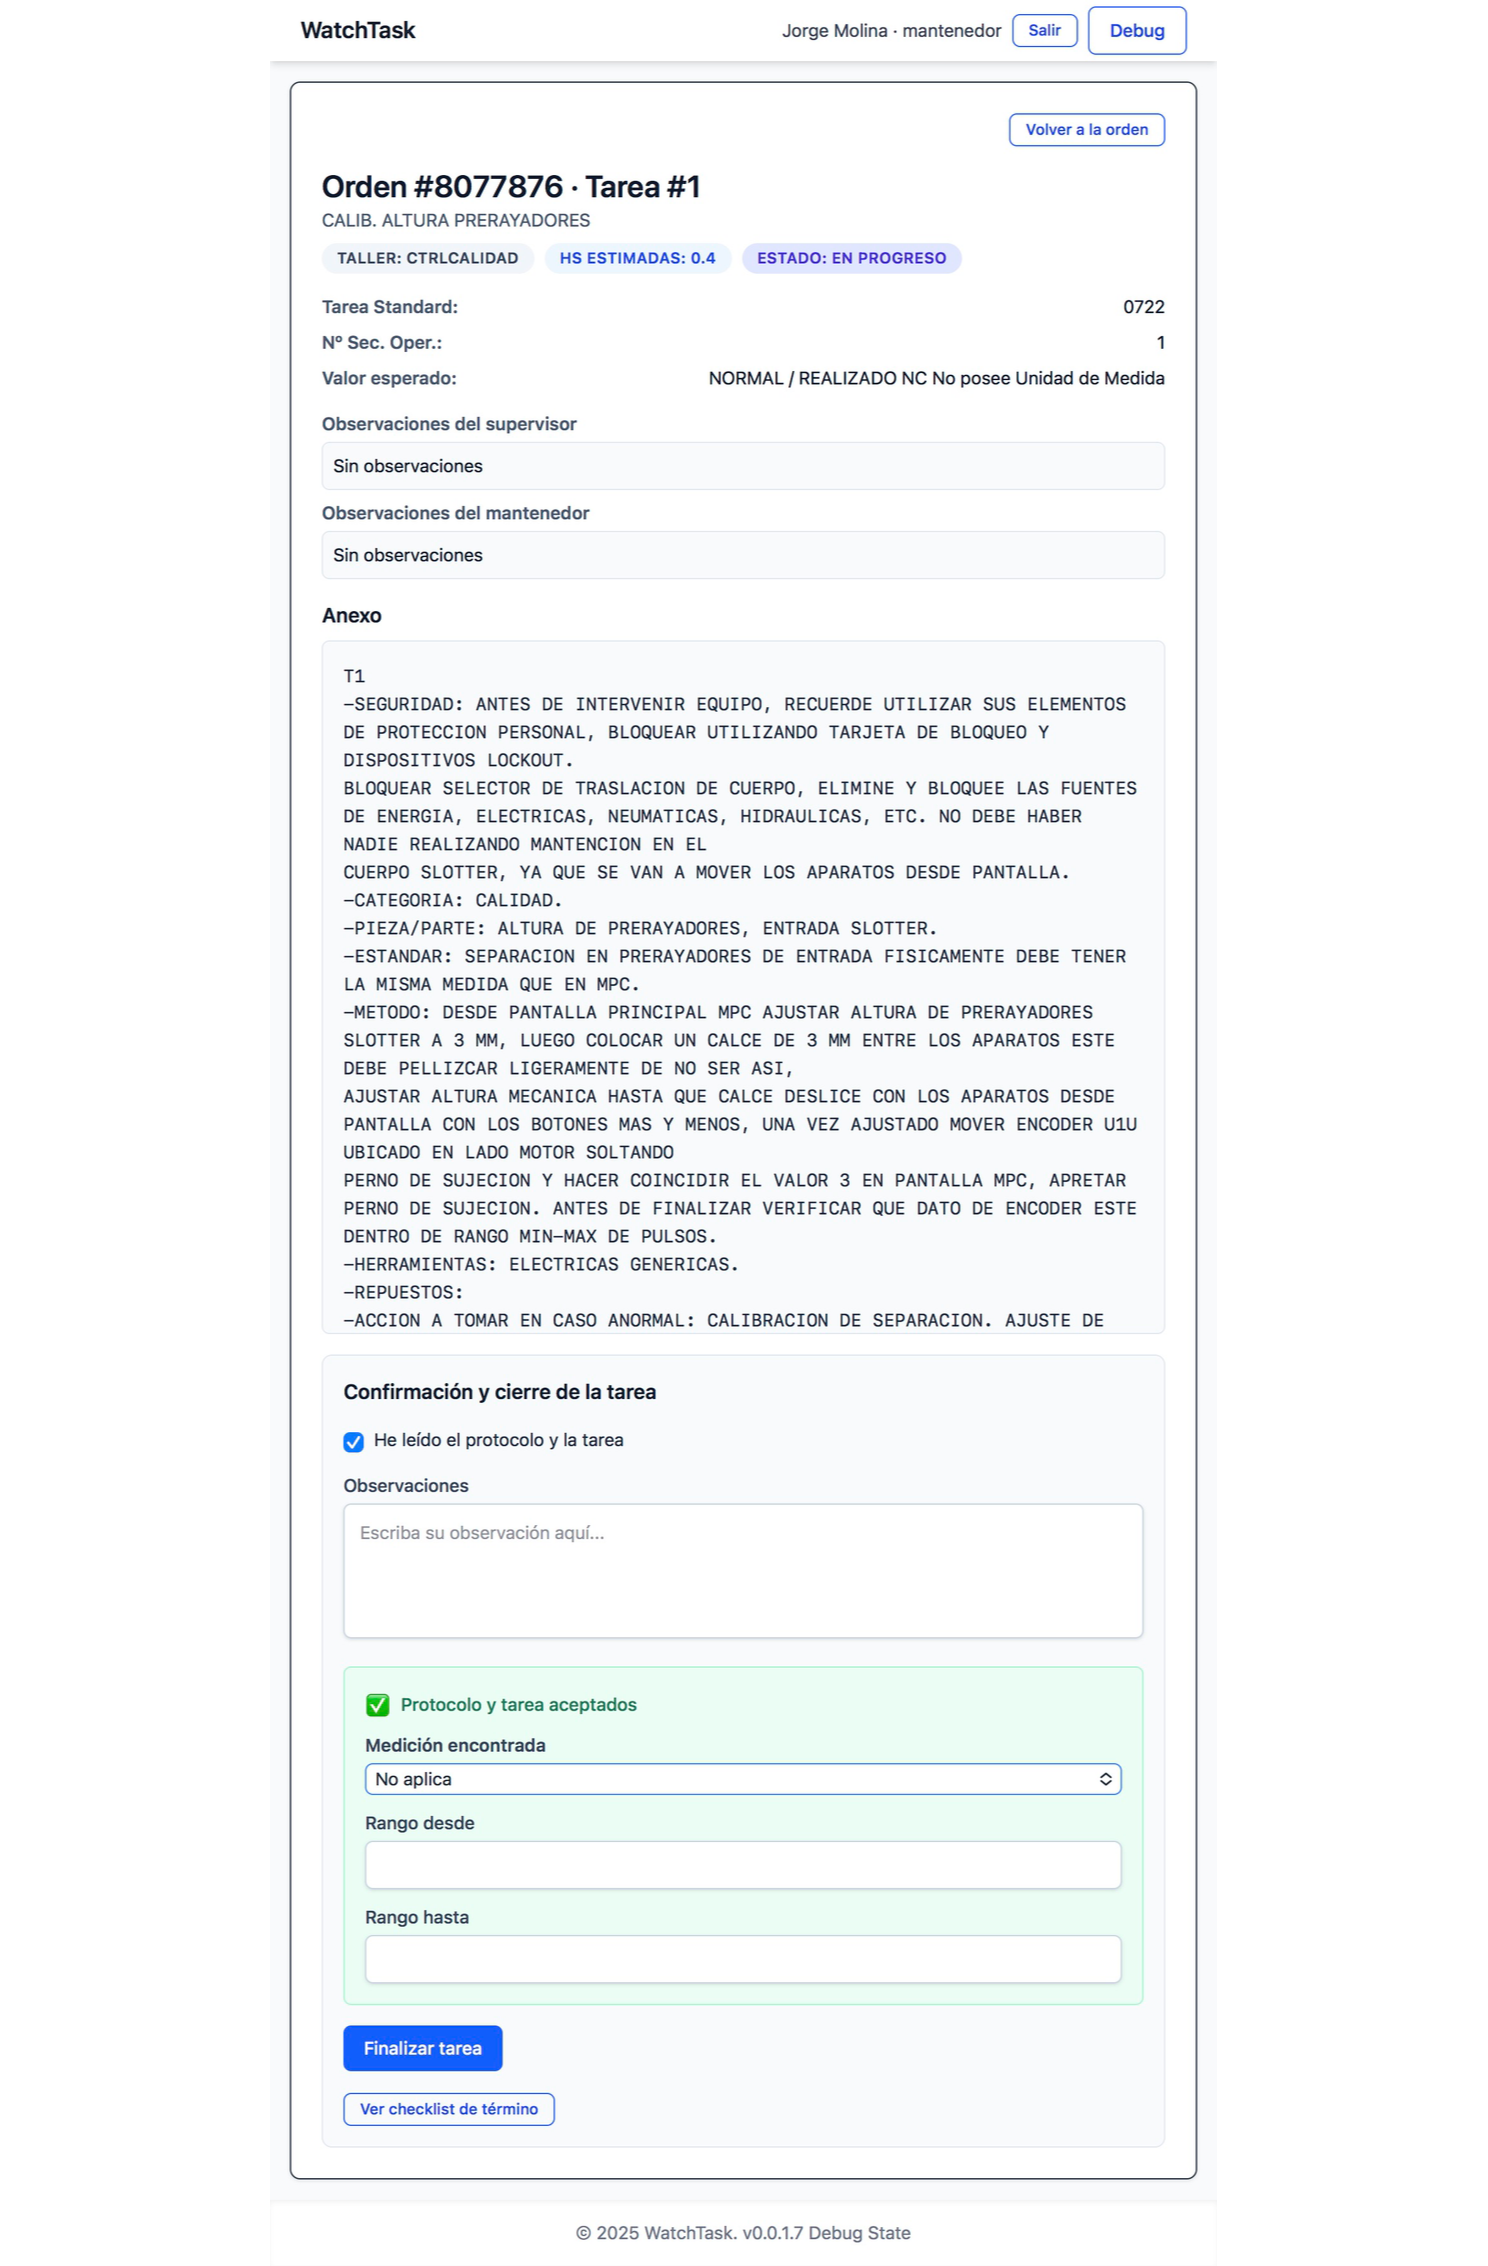
\includegraphics[width=1\textwidth]{data/Mantenedor_Task.png}
    \caption[\,Mantenedor: Vista de Tarea]{Interfaz de usuario con perfil Mantenedor, Vista de Tarea especifica de una orden.}
    \label{fig:[Mantenedor_Task]}
\end{figure}
\begin{figure}[h]
    \centering
    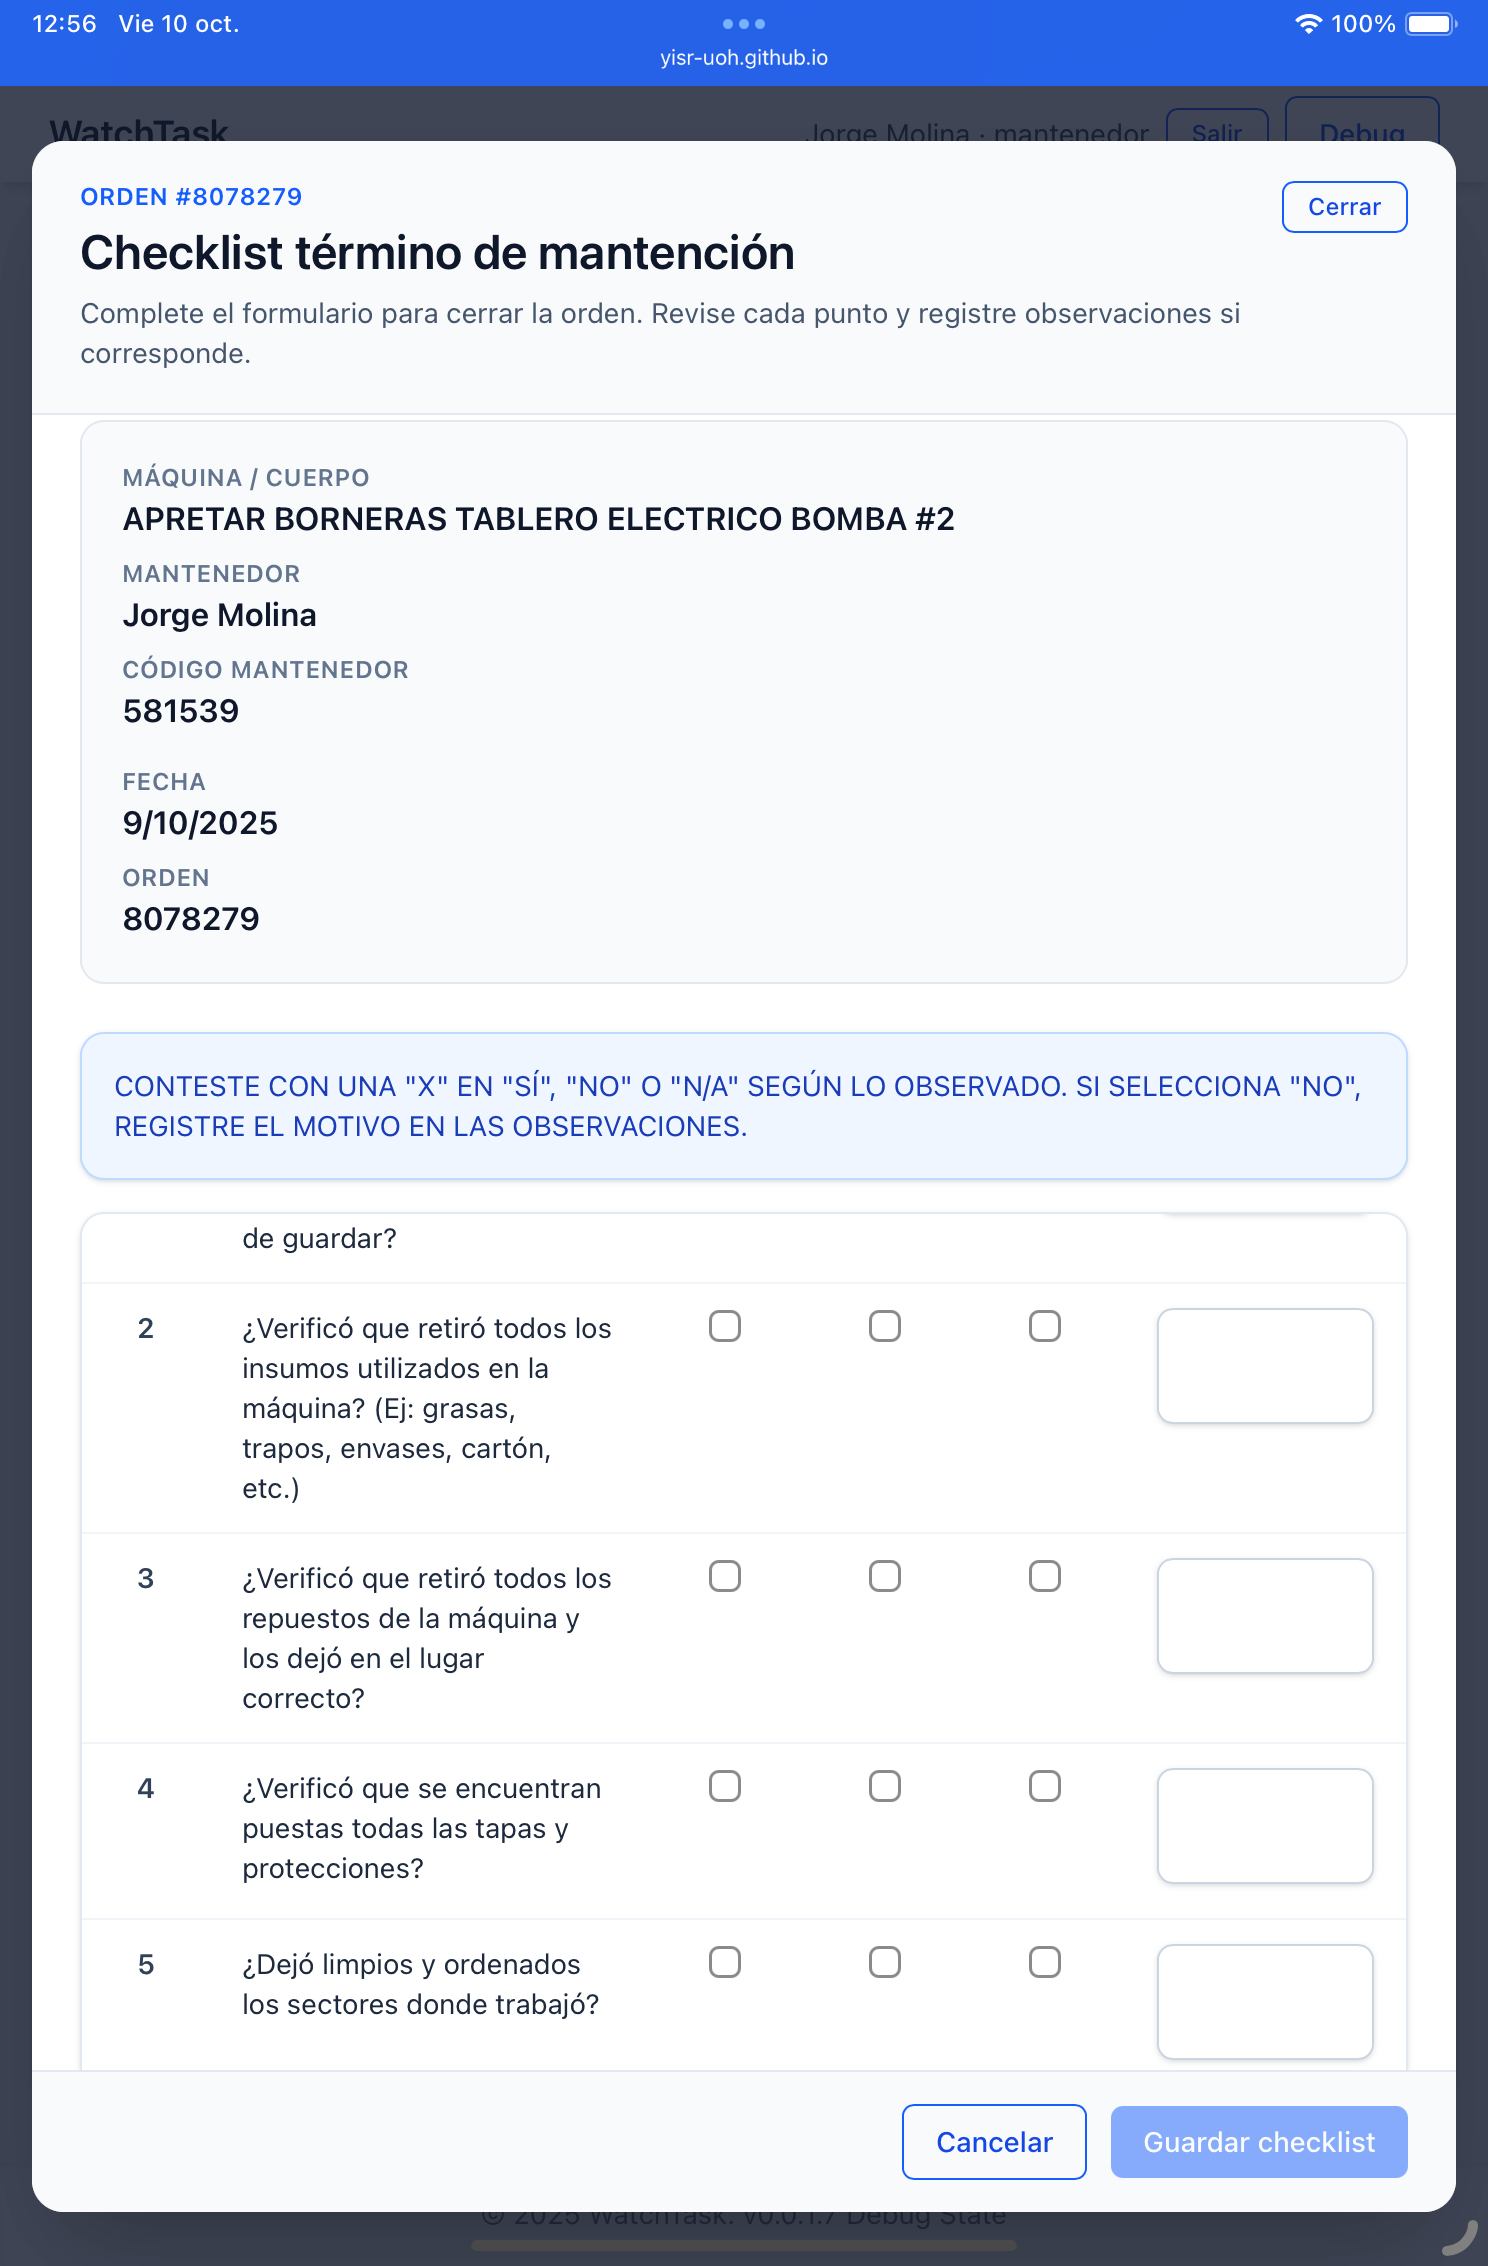
\includegraphics[width=1\textwidth]{data/Mantenedor_Checklist.png}
    \caption[\,Mantenedor: Checklist de término]{Interfaz de usuario con perfil Mantenedor, Vista de CheckList de termino de orden de mantenimiento.}
    \label{fig:[Mantenedor_ChechList]}
\end{figure}
\begin{figure}[h]
    \centering
    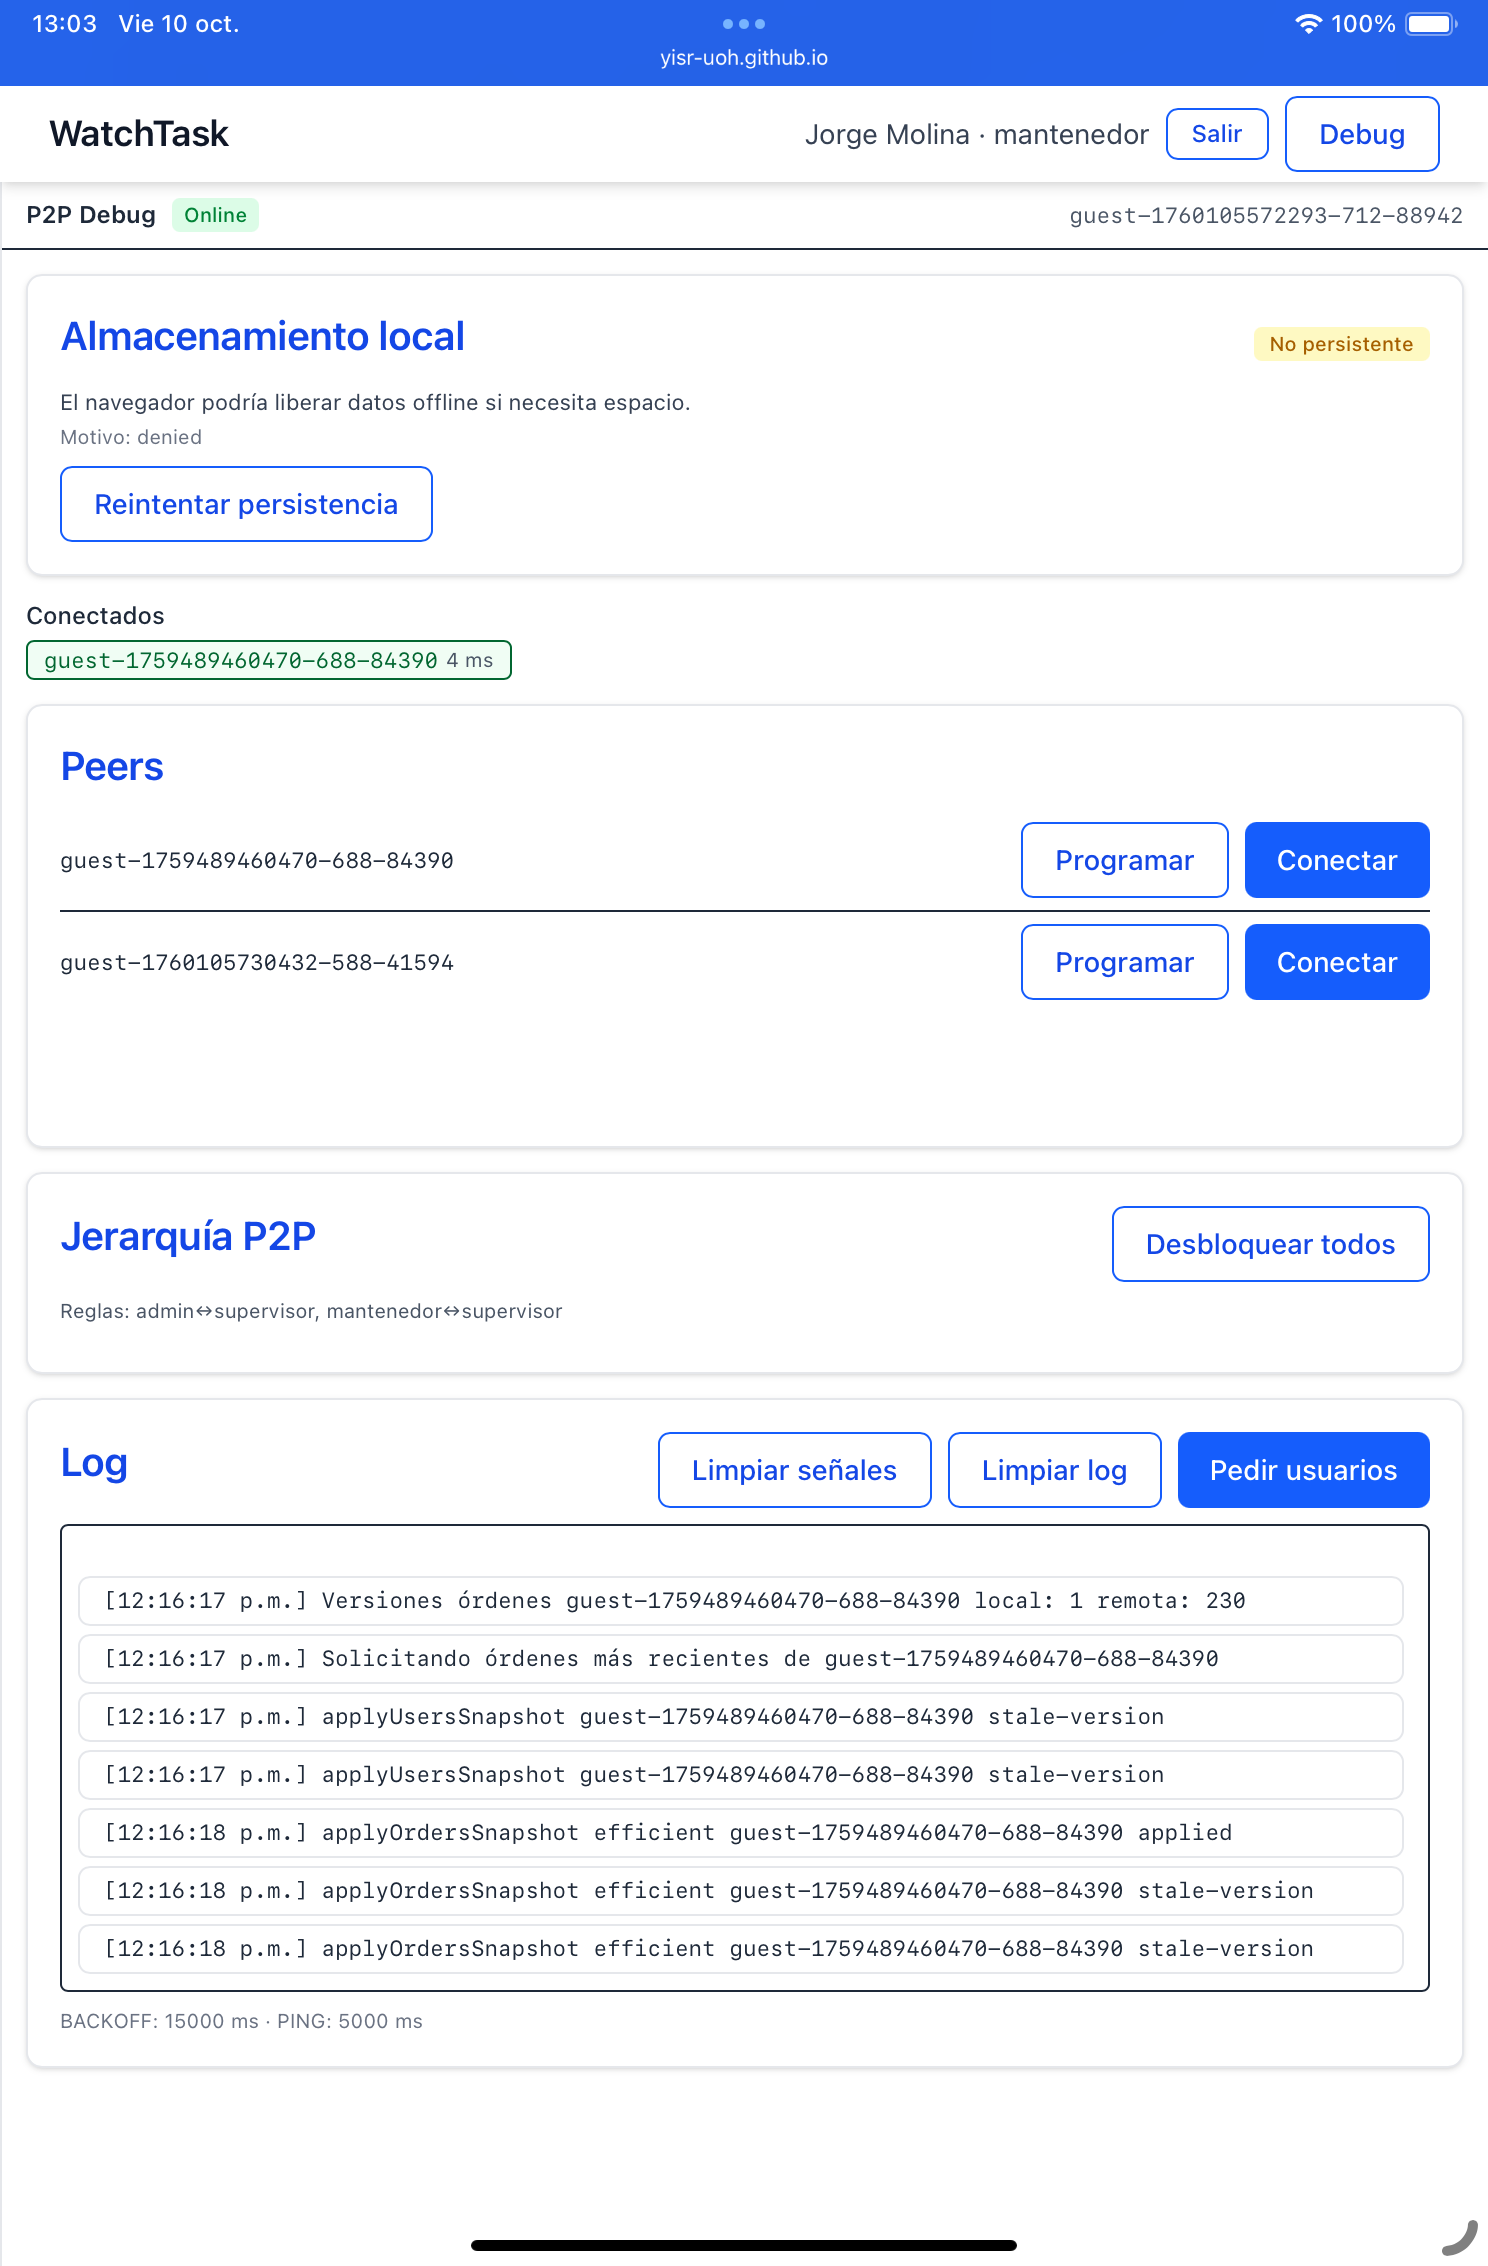
\includegraphics[width=1\textwidth]{data/Debug_Panel.png}
    \caption[\,Panel de depuración P2P]{Panel para revisar estado de conexiones entre peers, latencia, estado de red y persistencia de datos.}
    \label{fig:[Debug_Panel]}
\end{figure}



\chapter*{Glosario de Términos}
\addcontentsline{toc}{chapter}{Glosario de Términos}
\begin{itemize}
    \item BSON: Binary JSON, un formato de serialización de datos que extiende JSON para incluir tipos de datos adicionales y es utilizado por MongoDB para almacenar documentos.
    \item Responsive: Diseño web que permite que las aplicaciones se adapten a diferentes tamaños de pantalla y dispositivos, proporcionando una experiencia de usuario óptima en móviles, tablets y desktops .
\end{itemize}


\bibliographystyle{apalike}
\bibliography{bibliografia}
\addcontentsline{toc}{chapter}{Bibliografia}
\end{document}